%CS6240 Software Engineering project paper

% Ge Gao - Nov. 1, 2009

\documentclass[acmtocl]{acmtrans2m}
\usepackage{graphicx}

%\documentclass[acmtocl]{}
%\documentclass{article}
%\usepackage{times}
\newcommand{\BibTeX}{{\rm B\kern-.05em{\sc i\kern-.025em b}\kern-.08em
    T\kern-.1667em\lower.7ex\hbox{E}\kern-.125emX}}


\begin{document}

% Article top matter
\title{Enabling Efficient Go Game on Android Platform} %\LaTeX is a macro for printing the Latex logo
\author{
 Michael Skalak, Gu Lin, Ge Gao\\
Department of Computer Science\\
University of Virginia\\
\texttt{\{gl2hv, gg5j\}@virginia.edu}\\
}  %\texttt formats the text to a typewriter style font
\date{}  %\today is replaced with the current date

\maketitle

\begin{abstract}

\end{abstract}

\section{Introduction}
 
Human\&Computer interactive go game on cell phone is everywhere today. Our project's "bang for the buck" lies in connecting cell phone users to worldwide weichi players on the Internet in mobile manner and getting a good weichi assistantship on mobile device. This could not be achieved previously due to the relative isolation of individule cell phones from 3G resources and their limited computing capability, which could be overcomed by recent  achievements in wide coverage of the wireless network and 3G networks, ability of cell phones to acess Internet, open APIs of cell phone OS, etc.. Our project is on the way to take advantage of these achievements to upgrade cell phones' game playing environment.

Risks might include: 
 \begin{itemize}
  \item limited cell phone computing resources;
  \item open search algorithm;
  \item unfamiliar with KGS server's protocol;
  \item unfamiliar with Android development environment.
 \end{itemize}

\section{Background and Related Work}

\section{System Design}

\subsection{Requirements}

\begin{enumerate}
 \item To allow someone to play weichi go game anywhere with other remote players;
 \item To work as a game assistant recommending a good move.
\end{enumerate}


\subsection{Specifications}

Our system
\begin{enumerate}
 \item Provides an interface to allow mobile weichi players to manipulate a go board;
 \item Provides a go engine through which mobile weichi players send go instructions and get assistance for next move;
 \item Provides a platform to enable mobile weichi players to log on KGS GO server to play go against people all over the world. 
\end{enumerate}

\subsection{Design}

\begin{figure*}[t]
 \centering
 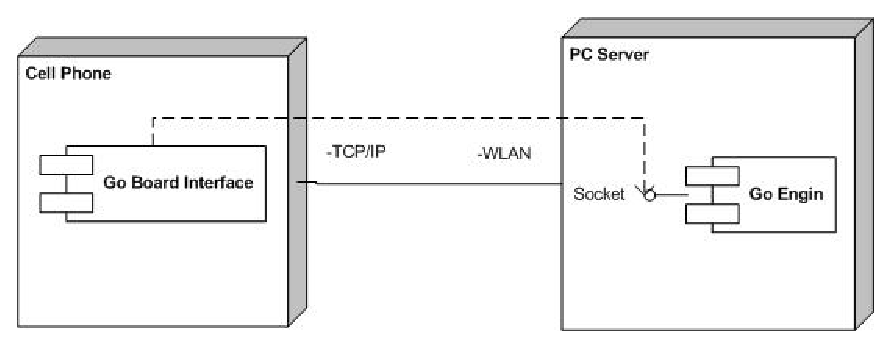
\includegraphics[width = \linewidth]{fig/deployment}
 % deployment.jpg: 549x201 pixel, 96dpi, 14.53x5.32 cm, bb=0 0 412 151
 \label{fig:deploy}
\end{figure*}

\begin{figure*}[t]
 \centering
 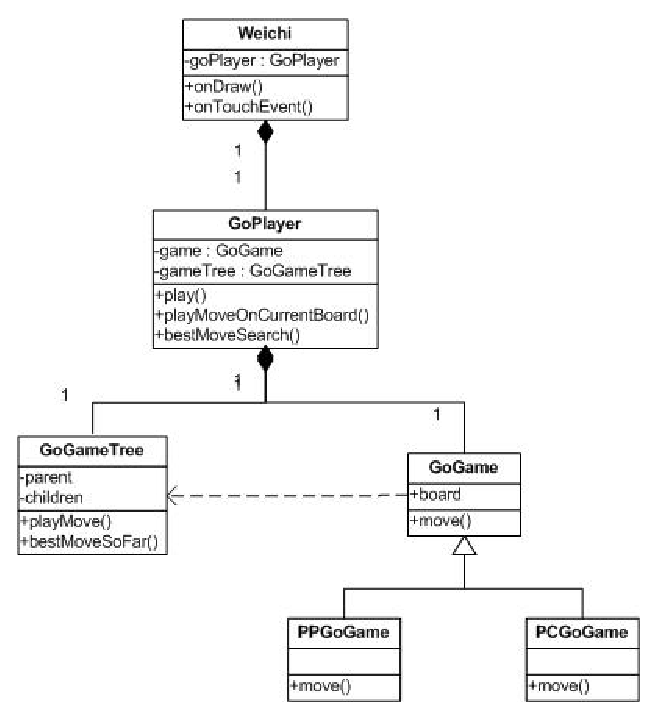
\includegraphics[width = \linewidth]{fig/class}
 % class.jpg: 399x438 pixel, 96dpi, 10.56x11.59 cm, bb=0 0 299 329
 \label{fig:class}
\end{figure*}


\section{Evaluation}

\subsection{Usage Scenarios}

\begin{figure*}[t]
 \centering
 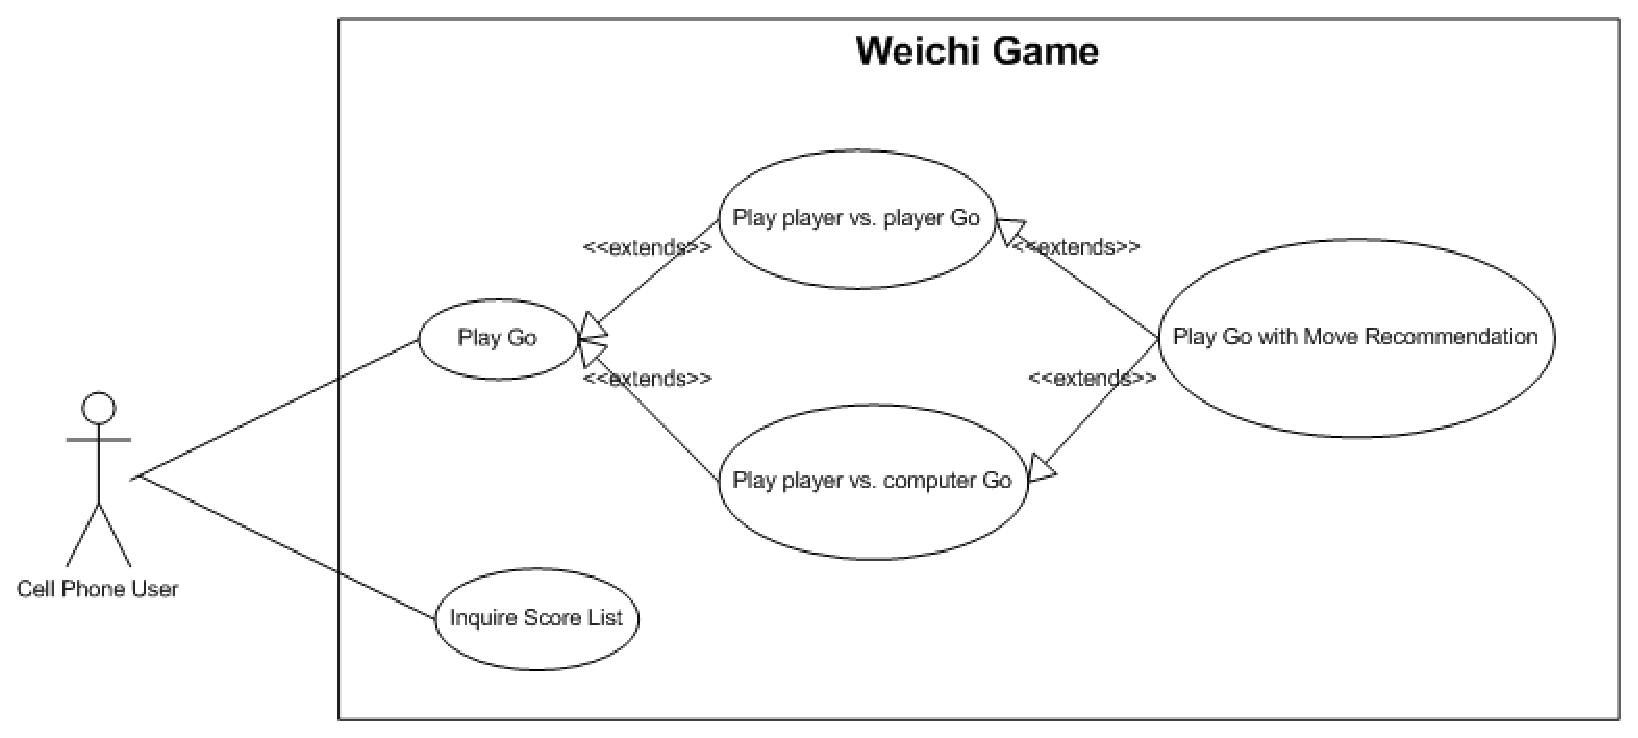
\includegraphics[width = \linewidth]{fig/user_case}
 % user_case.eps: 770x338 pixel, 300dpi, 6.52x2.86 cm, bb=0 0 770 338
 \label{fig:use}
\end{figure*}


\subsection{Test Results}

\section{Conclusion}



\begin{thebibliography}{9}
%The \bibitem is to start a new reference.  Ensure that the cite_key is
%unique.  You don't need to put each element on a new line, but I did
%simply for readability.


\end{thebibliography} %Must end the environment

\end{document}  %End of document.
